\section{Broken circuits}
\label{sec:broken}

In this section, we consider the case where the provided input 
$\mathcal{I}$ does not preserve the fibration symmetry 
\cite{Boldi2002,morone2020}. For this, we choose one node within 
the fiber to receive the input, which breaks
the fibration symmetry of the network. Note that we only provide 
input to mRNA nodes in the mRNA/Protein network representation.

\subsection{$|n = 1, \ell \rangle$ input-output circuit}
\label{ssec:broken_n1}

Considering the FFF broken circuit, we cannot reduce the network to the 
quotient form, since the fibration symmetry is broken by the 
input to $x_1^R$ only. Therefore, we need to verify all the possible 
regulation combinations for the input-output network shown 
in Fig.~\ref{fig:broken_n1}.

\begin{figure}[H]
    \centering
    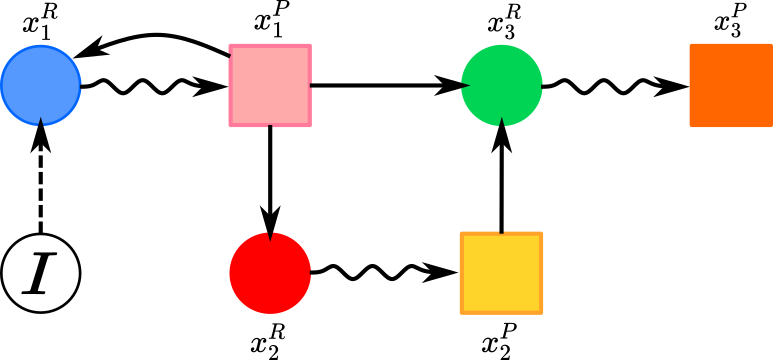
\includegraphics[scale=0.65]{figs/broken_n1.png}
    \caption{}
    \label{fig:broken_n1}
\end{figure}

\subsubsection{General vector fields}

The general possible dynamics restricted by
the topology of this network is given by the following system of 
admissible equations \cite{martin_ian_groupoids2006}:
\begin{equation} \label{eq:broken_n1_1}
    \begin{aligned}
        \dot{x}_1^R &= f_{x_1^R}(x_1^R, x_1^P, \mathcal{I})\\
        \dot{x}_1^P &= f_{x_1^P}(x_1^P, x_1^R)\\
        \dot{x}_2^R &= f_{x_2^R}(x_2^R, x_1^P)\\
        \dot{x}_2^P &= f_{x_2^P}(x_2^P, x_2^R)\\
        \dot{x}_3^R &= f_{x_3^R}(x_3^R, x_1^P, x_2^P)\\
        \dot{x}_3^P &= f_{x_3^P}(x_3^P, x_3^R)
    \end{aligned},
\end{equation}
where $\vec{F} = (f_{x_1^R}, f_{x_1^P}, f_{x_2^R}, f_{x_2^P}, 
f_{x_3^R}, f_{x_3^P})$ is 
the vector of nonlinear functions as described in 
section~\ref{sec:intro}. The Jacobian of this system is 
\begin{equation}
    J = 
    \begin{pmatrix}
        f_{x_1^R,x_1^R} & f_{x_1^R, x_1^P} & 0 & 0 & 0 & 0 \\
        f_{x_1^P,x_1^R} & f_{x_1^P,x_1^P} & 0 & 0 & 0 & 0 \\
        0 & f_{x_2^R,x_1^P} & f_{x_2^R,x_2^R} & 0 & 0 & 0 \\
        0 & 0 & f_{x_2^P,x_2^R} & f_{x_2^P,x_2^P} & 0 & 0 \\
        0 & f_{x_3^R,x_1^P} & 0 & f_{x_3^R,x_2^P} & f_{x_3^R,x_3^R} & 0 \\
        0 & 0 & 0 & 0 & f_{x_3^P,x_3^R} & f_{x_3^P,x_3^P} \\
    \end{pmatrix},
\end{equation} 
where the condition for stability of equilibria is defined over 
$f_{x_2^R,x_2^R}$, $f_{x_2^R,x_2^R}$, $f_{x_3^R,x_3^R}$ and 
$f_{x_3^P,x_3^P}$ and the eigenvalues of the $2 \times 2$ 
block matrix defined by the first rows and columns of the Jacobian. 
Moreover, the homeostasis matrix is given by
\begin{equation}
    H = 
    \begin{pmatrix}
        f_{x_1^P,x_1^R} & f_{x_1^P,x_1^P} & 0 & 0 & 0\\
        0 & f_{x_2^R,x_1^P} & f_{x_2^R,x_2^R} & 0 & 0\\
        0 & 0 & f_{x_2^P,x_2^R} & f_{x_2^P,x_2^P} & 0\\
        0 & f_{x_3^R,x_1^P} & 0 & f_{x_3^R,x_2^P} & f_{x_3^R,x_3^R}\\
        0 & 0 & 0 & 0 & f_{x_3^P,x_3^R} \\
    \end{pmatrix}.
\end{equation} 

\subsubsection{Special model}

Considering the $| n=1, \ell \rangle$ fiber circuits observed in 
the \textit{E. Coli} genetic regulatory network, we have two 
possibilities for the regulations within the fiber: the SAT-FFF 
and the UNSAT-FFF. For each one of the two 
possibilities there are 4 possibles combinations for the external
regulations to node $x_3^R$: two with equal 
types of regulations to the output node (Fig.~\ref{fig:combination_n1}a,b,e,f), 
and two for the case of alternated types of regulations
(Fig.~\ref{fig:combination_n1}c,d,g,h). 

\begin{figure}[H]
    \centering
    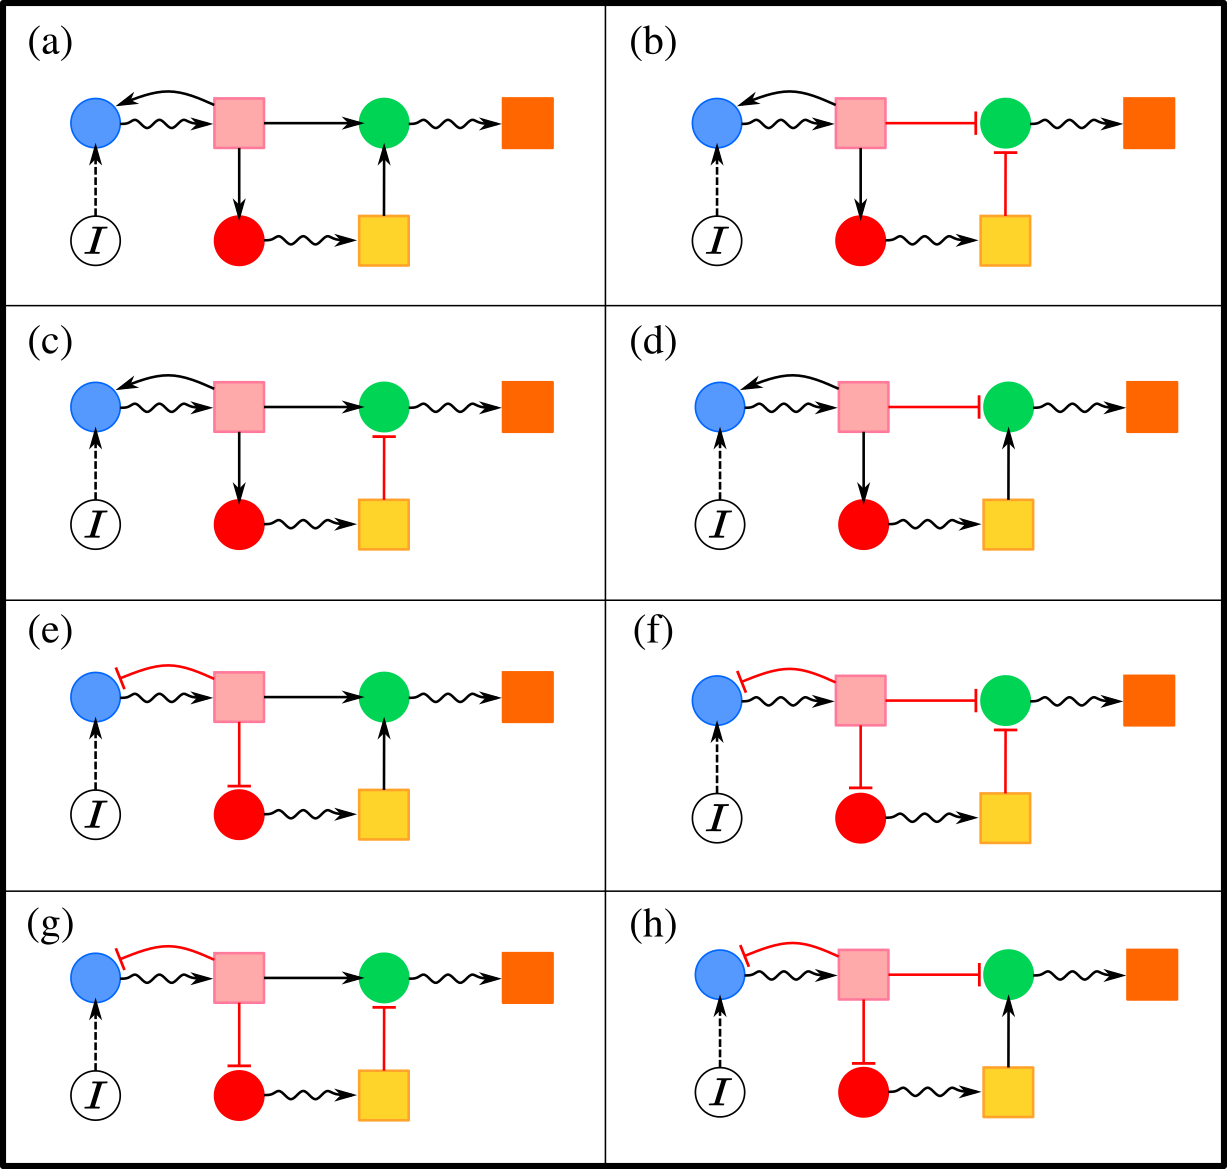
\includegraphics[scale=0.6]{figs/broken_n1_mosaic.png}
    \caption{}
    \label{fig:combination_n1}
\end{figure}

Now, considering the special equations \cite{stochs_gene_2005,homeostasis_antonelli2018}, we have the following core differential 
equations for all SAT-FFF and UNSAT-FFF circuits:

{
    \setlength{\tabcolsep}{12pt}
    \renewcommand{\arraystretch}{4.5}
\begin{table}[H]
    \centering
    \vspace{0.2cm}
    \hspace{-0.6cm}
    \begin{tabular}{|c|c|}
        \hline
        \textbf{SAT-FFF} & \textbf{UNSAT-FFF} \\
        \hline
        $\begin{aligned}
            \dot{x_1}^R &= -\delta_1 x_1^R + \gamma_1(1-S(x_1^P)) + I\\
            \dot{x_1}^P &= -\alpha_1 x_1^P + \beta_1 x_1^R\\
            \dot{x_2}^R &= -\delta_2 x_2^R + \gamma_2(1-S(x_1^P))\\
            \dot{x_2}^P &= -\alpha_2 x_2^P + \beta_2 x_2^R
        \end{aligned}$ & 
        $\begin{aligned}
            \dot{x_1}^R &= -\delta_1 x_1^R + \gamma_1 S(x_1^P) + I\\
            \dot{x_1}^P &= -\alpha_1 x_1^P + \beta_1 x_1^R\\
            \dot{x_2}^R &= -\delta_2 x_2^R + \gamma_2S(x_1^P)\\
            \dot{x_2}^P &= -\alpha_2 x_2^P + \beta_2 x_2^R
        \end{aligned}$ \\[0.70cm]
        \hline

    \end{tabular}
\end{table}
}

Therefore, we can list all combinations for the external 
regulated nodes $x_3^R$ and $x_3^P$ as 

{
\setlength{\tabcolsep}{10pt}
\renewcommand{\arraystretch}{3.0}
\begin{table}[H]
    \centering
    \vspace{0.2cm}
    \begin{tabular}{|c|c|}
        \hline
        \textbf{Circuit} & \textbf{SAT-FFF} \\
        \hline
        Fig.~\ref{fig:combination_n1}(a) & $\begin{aligned}
            \dot{x_3}^R &= -\delta_3 x_3^R + \gamma_3(1-T(x_1^P+x_2^P))\\
            \dot{x_3}^P &= -\alpha_3 x_3^P + \beta_3 x_3^R
        \end{aligned}$ \\[0.25cm]
        \hline
        Fig.~\ref{fig:combination_n1}(b) & $\begin{aligned}
            \dot{x_3}^R &= -\delta_3 x_3^R + \gamma_3 T(x_1^P+x_2^P)\\
            \dot{x_3}^P &= -\alpha_3 x_3^P + \beta_3 x_3^R
        \end{aligned}$ \\[0.25cm]
        \hline
        Fig.~\ref{fig:combination_n1}(d) & $\begin{aligned}
            \dot{x_3}^R &= -\delta_3 x_3^R + \gamma_3 S(x_1^P) + \gamma_3'(1 - S(x_2^P))\\
            \dot{x_3}^P &= -\alpha_3 x_3^P + \beta_3 x_3^R
        \end{aligned}$
         \\[0.25cm]
        \hline
        Fig.~\ref{fig:combination_n1}(c) & $\begin{aligned}
            \dot{x_3}^R &= -\delta_3 x_3^R + \gamma_3(1 - S(x_1^P)) + \gamma_3' S(x_2^P) \\
            \dot{x_3}^P &= -\alpha_3 x_3^P + \beta_3 x_3^R
        \end{aligned}$
         \\[0.25cm]
        \hline
    \end{tabular}
\end{table}
}

{
\setlength{\tabcolsep}{10pt}
\renewcommand{\arraystretch}{3.0}
\begin{table}[H]
    \centering
    \vspace{0.2cm}
    \hspace*{-1.5cm}
    \begin{tabular}{|c|c|}
        \hline
        \textbf{Circuit} & \textbf{UNSAT-FFF} \\
        \hline
        Fig.~\ref{fig:combination_n1}(e) & 
        $\begin{aligned}
            \dot{x_3}^R &= -\delta_3 x_3^R + \gamma_3(1-T(x_1^P+x_2^P))\\
            \dot{x_3}^P &= -\alpha_3 x_3^P + \beta_3 x_3^R
        \end{aligned}$ \\[0.25cm]
        \hline
        Fig.~\ref{fig:combination_n1}(f)  &
        $\begin{aligned}
            \dot{x_3}^R &= -\delta_3 x_3^R + \gamma_3T(x_1^P+x_2^P)\\
            \dot{x_3}^P &= -\alpha_3 x_3^P + \beta_3 x_3^R
        \end{aligned}$ \\[0.25cm]
        \hline
        Fig.~\ref{fig:combination_n1}(h)
        & $\begin{aligned}
            \dot{x_3}^R &= -\delta_3 x_3^R + \gamma_3 S(x_1^P) + \gamma_3'(1 - S(x_2^P))\\
            \dot{x_3}^P &= -\alpha_3 x_3^P + \beta_3 x_3^R
        \end{aligned}$ \\[0.25cm]
        \hline
        Fig.~\ref{fig:combination_n1}(g)
        & $\begin{aligned}
            \dot{x_3}^R &= -\delta_3 x_3^R + \gamma_3(1 - S(x_1^P)) + \gamma_3' S(x_2^P) \\
            \dot{x_3}^P &= -\alpha_3 x_3^P + \beta_3 x_3^R
        \end{aligned}$ \\[0.25cm]
        \hline
    \end{tabular}
\end{table}
}

\subsubsection{Stable equilibrium conditions}

The general form of the Jacobian assumes two different 
patterns according to the combination of regulations. These 
two forms are represented by $J_1$ and $J_2$ and are given 
as follows:
\begin{equation} \label{eq:jaco-special-1}
    J_1 = 
    \begin{pmatrix}
        -\delta_1 & \xi_1\gamma_1S'(x_1^P) & 0 & 0 & 0 & 0 \\
        \beta_1 & -\alpha_1 & 0 & 0 & 0 & 0 \\
        0 & \xi_1\gamma_2 S'(x_1^P) & -\delta_2 & 0 & 0 & 0 \\
        0 & 0 & \beta_2 & -\alpha_2 & 0 & 0 \\
        0 & \xi_2 \gamma_3 T'(x_1^P + x_2^P) & 0 & \xi_2 \gamma_3 T'(x_1^P + x_2^P) & -\delta_3 & 0 \\
        0 & 0 & 0 & 0 & \beta_3 & -\alpha_3 \\
    \end{pmatrix},
\end{equation}
and 
\begin{equation} \label{eq:jaco-special-2}
    J_2 = 
    \begin{pmatrix}
        -\delta_1 & \xi_1\gamma_1S'(x_1^P) & 0 & 0 & 0 & 0 \\
        \beta_1 & -\alpha_1 & 0 & 0 & 0 & 0 \\
        0 & \xi_1\gamma_2 S'(x_1^P) & -\delta_2 & 0 & 0 & 0 \\
        0 & 0 & \beta_2 & -\alpha_2 & 0 & 0 \\
        0 & \xi_2 \gamma_3 S'(x_1^P) & 0 & -\xi_2 \gamma_3 S'(x_2^P) & -\delta_3 & 0 \\
        0 & 0 & 0 & 0 & \beta_3 & -\alpha_3 \\
    \end{pmatrix},
\end{equation}
where we have $\xi_1, \xi_2 \in \{ -1, +1 \}$. $J_1$ and $J_2$ 
represent both SAT and UNSAT circuits depending on the combinations 
of $\xi_1$, while $\xi_2$ is related to the type of the external 
regulations. $S$ and $T$ are both Hill functions.

Now, define
\begin{equation}
K = 
    \begin{pmatrix}
        -\delta_1 & \xi_1\gamma_1S'(x_1^P) \\
        \beta_1 & -\alpha_1 \\
    \end{pmatrix},
\end{equation} 
such that we have
\begin{equation}
    \begin{aligned}
        \Delta_k &= det(K) = \alpha_1 \delta_1 - \xi_1 \beta_1 \gamma_1 S'(x_1^P)\\
        \tau_k &= Tr(K) = -(\alpha_1 + \delta_1)
    \end{aligned}.
\end{equation}

Since the matrix $K$ is the same for both forms of the 
Jacobian, we have that the stability conditions for $J_1$ 
and $J_2$ are the same. Thus,
{
    \setlength{\tabcolsep}{10pt}
    \renewcommand{\arraystretch}{3.0}
\begin{table}[H]
    \centering
    \begin{tabular}{|c|c|c|}
        \hline
        $-\delta_2 < 0$ & $-\delta_3 < 0$ & $-(\alpha_1 + \delta_1) < 0$ \\
        \hline
        $-\alpha_2 < 0$ & $-\alpha_3 < 0$ & $\alpha_1 \delta_1 - \xi_1 \beta_1 \gamma_1 S'(x_1^P) > 0$\\
        \hline
    \end{tabular}
\end{table}
}

Considering that all parameters are strictly positive, then all
conditions depending only on the parameters are satisfied. The 
last one depending on $S'(x^P)$ is always satisfied for 
$\xi_1 = +1$ (positive inner regulations). For the case 
$\xi_1 = -1$(negative inner regulations), the derivative of the Hill function must satisfy 
the relation
\begin{equation}
    S'(x_1^P) > -\dfrac{\alpha_1 \delta_1}{\beta_1 \gamma_1}.
\end{equation} 

\subsubsection{Infinitesimal homeostasis conditions}

Since the homeostasis matrix $H$ is not the same for $J_1$
and $J_2$, then we define $H_1$ and $H_2$ to distinguish between 
the two cases:
\begin{equation}
    H_1 = 
    \begin{pmatrix}
        \beta_1 & -\alpha_1 & 0 & 0 & 0  \\
        0 & \xi_1\gamma_2 S'(x_1^P) & -\delta_2 & 0 & 0 \\
        0 & 0 & \beta_2 & -\alpha_2 & 0 \\
        0 & \xi_2 \gamma_3 T'(x_1^P + x_2^P) & 0 & \xi_2 \gamma_3 T'(x_1^P + x_2^P) & -\delta_3 \\
        0 & 0 & 0 & 0 & \beta_3 \\
    \end{pmatrix},
\end{equation}
and 
\begin{equation}
    H_2 = 
    \begin{pmatrix}
        \beta_1 & -\alpha_1 & 0 & 0 & 0 \\
        0 & \xi_1\gamma_2 S'(x_1^P) & -\delta_2 & 0 & 0 \\
        0 & 0 & \beta_2 & -\alpha_2 & 0 \\
        0 & \xi_2 \gamma_3 S'(x_1^P) & 0 & -\xi_2 \gamma_3 S'(x_2^P) & -\delta_3 \\
        0 & 0 & 0 & 0 & \beta_3 \\
    \end{pmatrix},
\end{equation}

To facilitate the calculation of the determinant of the given 
matrices, we use the method used in section~\ref{sec:example}
to find the irreducible blocks of $H_{1,2}$ using the topology 
of the network.

There are only simple nodes in this network, and only three of 
them are super-simple nodes: $x_1^R, x_3^R, x_3^P$. Thus, each 
pair of super-simple nodes defines the subnetworks: 
$\mathcal{L}'(x_1^R, x_3^R)$ and $\mathcal{L}'(x_3^R, x_3^P)$. 
From these two subnetworks, we have 
the following infinitesimal homeostasis conditions:
\begin{equation}
    f_{x_3^P,x_3^R} = \beta_3(I_0) = 0,
\end{equation}
for both $H_1$ and $H_2$ combinations. However, we do not expect 
this to be satisfied because $\beta_i \neq 0$.

For the subnetwork $\mathcal{L}'(x_1^R, x_3^R)$, we have the 
following conditions. For $H_1$:
\begin{equation}
    det 
    \begin{pmatrix}
        \beta_1 & -\alpha_1 & 0 & 0  \\
        0 & \xi_1\gamma_2 S'(x_1^P) & -\delta_2 & 0 \\
        0 & 0 & \beta_2 & -\alpha_2 \\
        0 & \xi_2 \gamma_3 T'(x_1^P + x_2^P) & 0 & \xi_2 \gamma_3 T'(x_1^P + x_2^P) \\
    \end{pmatrix}(I_0) = 0,
\end{equation}
which gives us the condition
\begin{equation}
    \beta_1(\xi_1 \xi_2 \gamma_2 \gamma_3 \beta_2 S'(x_1^P)
    T'(x_1^P + x_2^P) + \xi_2 \delta_2 \alpha_2 \gamma_3 
    T'(x_1^P + x_2^P)) = 0,
\end{equation}
and considering that $\beta_1 \neq 0$, we have 
\begin{equation}
    \xi_1 \xi_2 \gamma_2 \gamma_3 \beta_2 S'(x_1^P)
    T'(x_1^P + x_2^P) + \xi_2 \delta_2 \alpha_2 \gamma_3 
    T'(x_1^P + x_2^P) = 0,
\end{equation}
or
\begin{equation}
    T'(x_1^P + x_2^P)(\delta_2 \alpha_2 + 
    \xi_1 \gamma_2 \beta_2 S'(x_1^P)) = 0
\end{equation}

Following the same procedure for matrix $H_2$, we have 
\begin{equation}
    -\xi_1 \xi_2 \gamma_2 \gamma_3' \beta_2 S'(x_1^P)
    S'(x_2^P) + \xi_2 \delta_2 \alpha_2 \gamma_3 
    S'(x_1^P) = 0,
\end{equation}
or 
\begin{equation}
    S'(x_1^P)(\delta_2 \alpha_2 \gamma_3 - \xi_1 \gamma_2 
    \gamma_3' \beta_2 S'(x_2^P)) = 0.
\end{equation}


\subsection{$|\phi_2, \ell \rangle$ input-output circuit}
\label{ssec:broken-fibo}

Here, we consider the case where the given input $\mathcal{I}$
turns the Fibonacci fiber of golden ratio $\phi_2$ into a broken 
symmetric circuit. For this, only the dynamics of node $x_2^R$ 
from Fig.~\ref{fig:broken_fibo} depends explicitly on the 
input $\mathcal{I}$. Thus, we cannot reduce the circuit to its 
quotient form.

\begin{figure}[H]
    \centering
    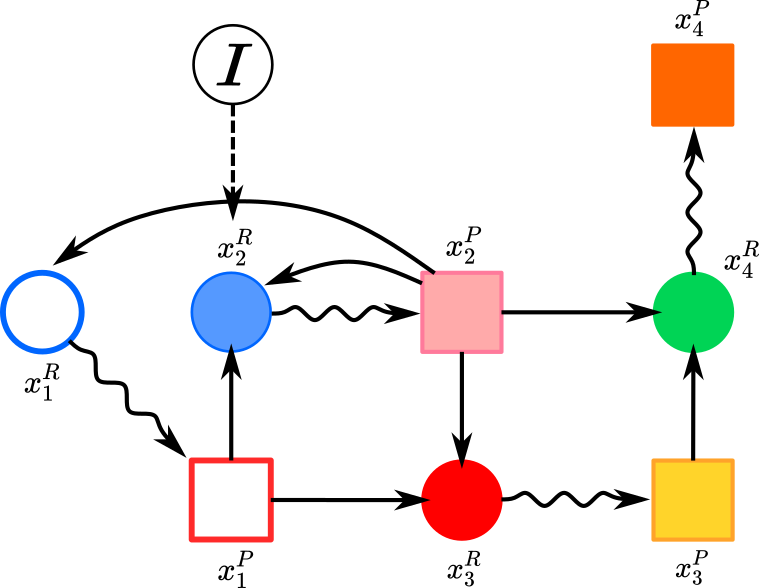
\includegraphics[scale=0.65]{figs/broken_fibo_1.png}
    \caption{}
    \label{fig:broken_fibo}
\end{figure}

\subsubsection{General vector fields}

The general possible dynamics restricted by
the topology of this network is given by the following system of 
admissible equations:
\begin{equation}
    \begin{aligned}
        \dot{x}_1^R &= f_{x_1^R}(x_1^R, x_2^P)\\
        \dot{x}_1^P &= f_{x_1^P}(x_1^P, x_1^R)\\
        \dot{x}_2^R &= f_{x_2^R}(x_2^R, x_1^P, x_2^P, \mathcal{I})\\
        \dot{x}_2^P &= f_{x_2^P}(x_2^P, x_2^R)\\
        \dot{x}_3^R &= f_{x_3^R}(x_3^R, x_1^P, x_2^P)\\
        \dot{x}_3^P &= f_{x_3^P}(x_3^P, x_3^R)\\
        \dot{x}_4^R &= f_{x_4^R}(x_4^R, x_2^P, x_3^P)\\
        \dot{x}_4^P &= f_{x_4^P}(x_4^P, x_4^R)
    \end{aligned},
\end{equation}
where $\vec{F} = (f_{x_1^R}, f_{x_1^P}, f_{x_2^R}, f_{x_2^P}, 
f_{x_3^R}, f_{x_3^P}, f_{x_4^R}, f_{x_4^P})$ is 
the vector of nonlinear functions as described in 
section~\ref{sec:intro}. The Jacobian of this system is 
\begin{equation}
    J = 
    \begin{pmatrix}
        f_{x_1^R,x_1^R} & 0 & 0 & f_{x_1^R, x_2^P} & 0 & 0 & 0 & 0 \\
        f_{x_1^P,x_1^R} & f_{x_1^P,x_1^P} & 0 & 0 & 0 & 0 & 0 & 0 \\
        0 & f_{x_2^R,x_1^P} & f_{x_2^R,x_2^R} & f_{x_1^P, x_2^P} & 0 & 0 & 0 & 0 \\
        0 & 0 & f_{x_2^P,x_2^R} & f_{x_2^P,x_2^P} & 0 & 0 & 0 & 0 \\
        0 & f_{x_3^R,x_1^P} & 0 & f_{x_3^R,x_2^P} & f_{x_3^R,x_3^R} & 0 & 0 & 0 \\
        0 & 0 & 0 & 0 & f_{x_3^P,x_3^R} & f_{x_3^P,x_3^P} & 0 & 0 \\
        0 & 0 & 0 & f_{x_4^R,x_2^P} & 0 & f_{x_4^R,x_3^P} & f_{x_4^R,x_4^R} & 0 \\
        0 & 0 & 0 & 0 & 0 & 0 & f_{x_4^P, x_4^R} & f_{x_4^P, x_4^P} \\
    \end{pmatrix},
\end{equation} 
where the condition for stability of equilibria is defined over 
$f_{x_3^R,x_3^R}$, $f_{x_3^P,x_3^P}$, $f_{x_4^R,x_4^R}$ and 
$f_{x_4^P,x_4^P}$ and the eigenvalues of the $4 \times 4$ 
block matrix defined by the first rows and columns of the Jacobian. 
Moreover, the homeostasis matrix is given by
\begin{equation}
    H = 
    \begin{pmatrix}
        f_{x_1^R,x_1^R} & 0 & 0 & f_{x_1^R, x_2^P} & 0 & 0 & 0 \\
        f_{x_1^P,x_1^R} & f_{x_1^P,x_1^P} & 0 & 0 & 0 & 0 & 0 \\
        0 & 0 & f_{x_2^P,x_2^R} & f_{x_2^P,x_2^P} & 0 & 0 & 0 \\
        0 & f_{x_3^R,x_1^P} & 0 & f_{x_3^R,x_2^P} & f_{x_3^R,x_3^R} & 0 & 0 \\
        0 & 0 & 0 & 0 & f_{x_3^P,x_3^R} & f_{x_3^P,x_3^P} & 0 \\
        0 & 0 & 0 & f_{x_4^R,x_2^P} & 0 & f_{x_4^R,x_3^P} & f_{x_4^R,x_4^R} \\
        0 & 0 & 0 & 0 & 0 & 0 & f_{x_4^P, x_4^R} \\
    \end{pmatrix}.
\end{equation} 

\subsubsection{Special model}

Considering the genes $uxuR$, $lgoR$ and $exuR$ in the 
\textit{E.Coli} bacteria, these genes belong to the only Fibonacci $\phi_2$
circuit of the bacteria's genetic network, and they only regulate 
themselves with negative regulations. Therefore, we have four possible 
combinations by changing the regulations to node $x_4^R$ in 
Fig.~\ref{fig:broken_fibo}. These combinations are shown in 
Fig.~\ref{fig:fibo-combinations}.

\begin{figure}[H]
    \centering
    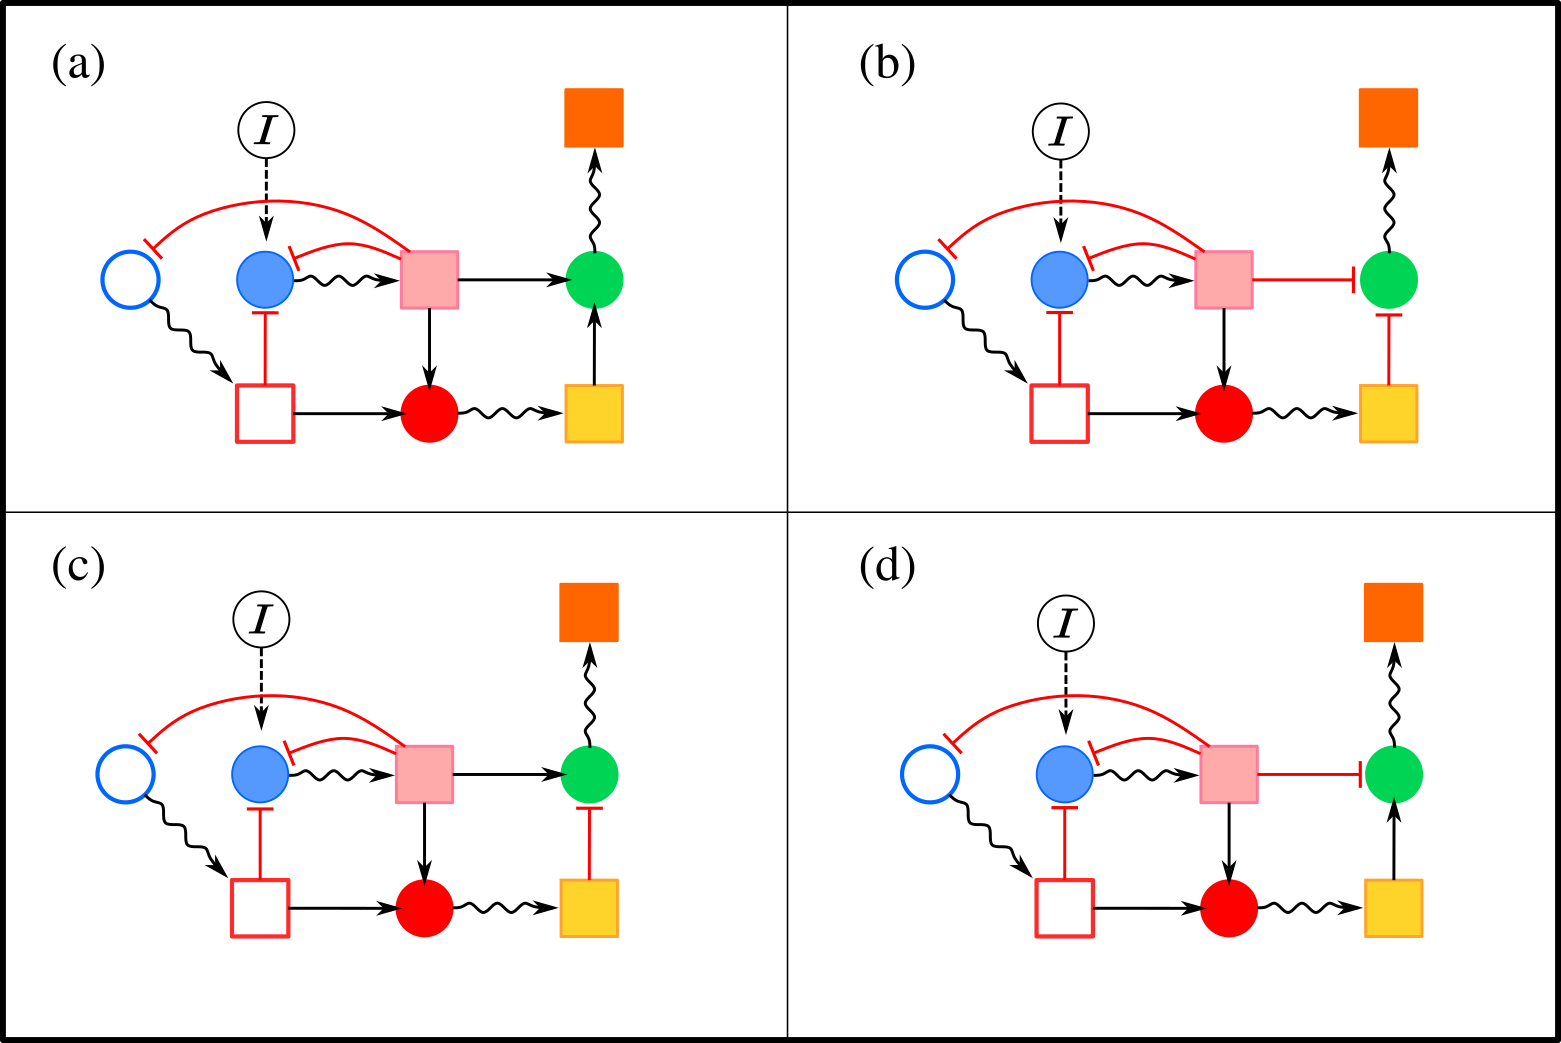
\includegraphics[scale=0.6]{figs/broken_fibo_mosaic.png}
    \caption{}
    \label{fig:fibo-combinations}
\end{figure}

Now, considering the special equations \cite{stochs_gene_2005}, 
we have the following core differential equations for 
the $uxuR$-$lgoR$-$exuR$ circuit:

{
    \setlength{\tabcolsep}{12pt}
    \renewcommand{\arraystretch}{4.5}
\begin{table}[H]
    \centering
    \vspace{0.2cm}
    \hspace{-0.6cm}
    \begin{tabular}{|c|}
        \hline
        \textbf{$uxuR$-$lgoR$-$exuR$ circuit} \\
        \hline
        $\begin{aligned}
            \dot{x_1}^R &= -\delta_1 x_1^R + \gamma_1S(x_1^P)\\
            \dot{x_1}^P &= -\alpha_1 x_1^P + \beta_1 x_1^R\\
            \dot{x_2}^R &= -\delta_2 x_2^R + \gamma_2T(x_1^P+x_2^P) + \mathcal{I}\\
            \dot{x_2}^P &= -\alpha_2 x_2^P + \beta_2 x_2^R\\
            \dot{x_3}^R &= -\delta_3 x_3^R + \gamma_3T(x_1^P+x_2^P) \\
            \dot{x_3}^P &= -\alpha_3 x_3^P + \beta_3 x_3^R
        \end{aligned}$  \\[1.250cm]
        \hline

    \end{tabular}
\end{table}
}

Therefore, we can list all combinations for the external 
regulated nodes $x_4^R$ and $x_4^P$ as 

{
\setlength{\tabcolsep}{10pt}
\renewcommand{\arraystretch}{3.0}
\begin{table}[H]
    \centering
    \vspace{0.2cm}
    \hspace*{-0.75cm}
    \begin{tabular}{|c|c|}
        \hline
        \textbf{Circuit} & \textbf{$uxuR$-$lgoR$-$exuR$ circuit} \\
        \hline
        Fig.~\ref{fig:fibo-combinations}(a) & $\begin{aligned}
            \dot{x_4}^R &= -\delta_4 x_4^R + \gamma_4(1-T(x_2^P+x_3^P))\\
            \dot{x_4}^P &= -\alpha_4 x_4^P + \beta_4 x_4^R
        \end{aligned}$  \\[0.25cm]
        \hline
        Fig.~\ref{fig:fibo-combinations}(b) & $\begin{aligned}
            \dot{x_4}^R &= -\delta_4 x_4^R + \gamma_4 T(x_2^P+x_3^P)\\
            \dot{x_4}^P &= -\alpha_4 x_4^P + \beta_4 x_4^R
        \end{aligned}$  \\[0.25cm]
        \hline
        Fig.~\ref{fig:fibo-combinations}(d) & $\begin{aligned}
            \dot{x_4}^R &= -\delta_4 x_4^R + \gamma_4 S(x_2^P) + \gamma_4'(1 - S(x_3^P))\\
            \dot{x_4}^P &= -\alpha_4 x_4^P + \beta_4 x_4^R
        \end{aligned}$ \\[0.25cm]
        \hline
        Fig.~\ref{fig:fibo-combinations}(c) & $\begin{aligned}
            \dot{x_4}^R &= -\delta_4 x_4^R + \gamma_4(1 - S(x_2^P)) + \gamma_4' S(x_3^P) \\
            \dot{x_4}^P &= -\alpha_4 x_4^P + \beta_4 x_4^R
        \end{aligned}$ \\[0.25cm]
        \hline
    \end{tabular}
\end{table}
}

\subsubsection{Stable equilibrium conditions}

The Jacobian of the system is a $8 \times 8$ matrix where the 
first six rows and columns are the same for all the 4 possible 
circuits. Considering the two forms $J_1$ and $J_2$ for the 
Jacobian, we have 
\begin{equation}
    J_1 = 
    \begin{pmatrix}
        -\delta_1 & 0 & 0 & \gamma_1 S'(x_2^P) & 0 & 0 & 0 & 0 \\
        \beta_1 & -\alpha_1 & 0 & 0 & 0 & 0 & 0 & 0 \\
        0 & \gamma_2 T'(x_1^P + x_2^P) & -\delta_2 & \gamma_2 T'(x_1^P + x_2^P) & 0 & 0 & 0 & 0 \\
        0 & 0 & \beta_2 & -\alpha_1 & 0 & 0 & 0 & 0 \\
        0 & \gamma_3 T'(x_1^P + x_2^P) & 0 & \gamma_3 T'(x_1^P + x_2^P) & -\delta_3 & 0 & 0 & 0 \\
        0 & 0 & 0 & 0 & \beta_3 & -\alpha_3 & 0 & 0 \\
        0 & 0 & 0 & \xi_1 \gamma_4 T'(x_2^P + x_3^P) & 0 & \xi_1 \gamma_4 T'(x_2^P + x_3^P) & -\delta_4 & 0 \\
        0 & 0 & 0 & 0 & 0 & 0 & \beta_4 & -\alpha_4 \\
    \end{pmatrix},
\end{equation} 
and 
\begin{equation}
    J_2 = 
    \begin{pmatrix}
        -\delta_1 & 0 & 0 & \gamma_1 S'(x_2^P) & 0 & 0 & 0 & 0 \\
        \beta_1 & -\alpha_1 & 0 & 0 & 0 & 0 & 0 & 0 \\
        0 & \gamma_2 T'(x_1^P + x_2^P) & -\delta_2 & \gamma_2 T'(x_1^P + x_2^P) & 0 & 0 & 0 & 0 \\
        0 & 0 & \beta_2 & -\alpha_1 & 0 & 0 & 0 & 0 \\
        0 & \gamma_3 T'(x_1^P + x_2^P) & 0 & \gamma_3 T'(x_1^P + x_2^P) & -\delta_3 & 0 & 0 & 0 \\
        0 & 0 & 0 & 0 & \beta_3 & -\alpha_3 & 0 & 0 \\
        0 & 0 & 0 & \xi_1 \gamma_4 S'(x_2^P) & 0 & -\xi_1 \gamma_4 S'(x_3^P) & -\delta_4 & 0 \\
        0 & 0 & 0 & 0 & 0 & 0 & \beta_4 & -\alpha_4 \\
    \end{pmatrix},
\end{equation} 
where $\xi_1 \in \{ -1, +1 \}$.

Now, define
\begin{equation}
K = 
    \begin{pmatrix}
        -\delta_1 & 0 & 0 & \gamma_1S'(x_1^P) \\
        \beta_1 & -\alpha_1 & 0 & 0 \\
        0 & \gamma_2 T'(x_1^P + x_2^P) & -\delta_2 & \gamma_2 T'(x_1^P + x_2^P) \\
        0 & 0 & \beta_2 & -\alpha_2 \\
    \end{pmatrix}.
\end{equation}

The stability analysis for the Jacobian $J$ of this system is more 
complex, since we have a block matrix of dimension $4 \times 4$. 
The other blocks contain in each one only one element.
Therefore, for the existence of a stable equilibrium point we 
require the partial requirements:
{
    \setlength{\tabcolsep}{10pt}
    \renewcommand{\arraystretch}{3.0}
\begin{table}[H]
    \centering
    \begin{tabular}{|c|c|c|}
        \hline
        $-\delta_3 < 0$ & $-\delta_4 < 0$  \\
        \hline
        $-\alpha_3 < 0$ & $-\alpha_4 < 0$ \\
        \hline
    \end{tabular}.
\end{table}
}
Moreover, we require that the real part of the eigenvalues of 
matrix $K$ are negative. The eigenvalues of $J$ are the roots
of the characteristic polynomial
\begin{equation}
    P(\lambda) = A + B\lambda + C\lambda^2 + D\lambda^3 + E\lambda^4,
\end{equation}
where we find
\begin{equation}
    \begin{aligned}
        A &= \delta_1 \alpha_1 (A' + \delta_2 \alpha_2) + B'\\
        B &= [\delta_1 \alpha_1(\alpha_2 + \delta_2) + \delta_2 \alpha_2(\alpha_1 + \delta_1)]
        + A'(\alpha_1 + \delta_1)\\
        C &= A' + [\delta_1 \alpha_1 + \delta_2 \alpha_2 + (\alpha_1 + \delta_1)(\alpha_2 + \delta_2)]\\
        D &= \delta_1 + \delta_2 + \alpha_1 + \alpha_2\\
        E & = 1
    \end{aligned}
\end{equation}
with 
\begin{equation}
    \begin{aligned}
        A' &= -\gamma_2 \beta_2 T'(x_1^P + x_2^P) \\
        B' &= -\gamma_1 \gamma_2 \beta_1 \beta_2 S'(x_2^P)T'(x_1^P + x_2^P)\\
    \end{aligned}.
\end{equation}

\subsubsection{Infinitesimal homeostasis conditions}

We obtain the infinitesimal homeostasis conditions by using 
the algorithm provided in \cite{wang2021}. For this circuit, all
nodes are simple, whereas four are super-simple: $x_2^R, x_2^P,
x_4^R$ and $x_4^P$. Therefore, we can find the subnetworks for 
the pairs of super-simple nodes: $\mathcal{L}'(x_2^R, x_2^P)$,
$\mathcal{L}'(x_2^P, x_4^R)$ and $\mathcal{L}'(x_4^R, x_4^P)$.
The infinitesimal homeostasis conditions for 
$\mathcal{L}'(x_2^R, x_2^P)$ and $\mathcal{L}'(x_4^R, x_4^P)$
are, respectively, $\beta_2(I_0) = 0$ and $\beta_4(I_0) = 0$,
which are not feasible since $\beta_i \neq 0$ for the special model.

For the subnetwork $\mathcal{L}'(x_2^P, x_4^R)$ we have the 
following homeostasis matrices 
\begin{equation}
    \begin{split}
    &H_1(\mathcal{L}'(x_2^P, x_4^R)) =\\
    & \begin{pmatrix}
        -\delta_1 & 0 & \gamma_1 S'(x_2^P) & 0 & 0 \\
        \beta_1 & -\alpha_1 & 0 & 0 & 0 \\
        0 & \gamma_3T'(x_1^P + x_2^P) & \gamma_3T'(x_1^P + x_2^P) & -\delta_3 & 0 \\
        0 & 0 & 0 & \beta_3 & -\alpha_3 \\
        0 & 0 & \xi_1 \gamma_4 T'(x_2^P + x_3^P) & 0 & \xi_1 \gamma_4 T'(x_2^P + x_3^P) \\
    \end{pmatrix}
    \end{split},
\end{equation} 
and 
\begin{equation}
    \begin{split}
    &H_2(\mathcal{L}'(x_2^P, x_4^R)) =\\
    &\begin{pmatrix}
        -\delta_1 & 0 & \gamma_1 S'(x_2^P) & 0 & 0 \\
        \beta_1 & -\alpha_1 & 0 & 0 & 0 \\
        0 & \gamma_3T'(x_1^P + x_2^P) & \gamma_3T'(x_1^P + x_2^P) & -\delta_3 & 0 \\
        0 & 0 & 0 & \beta_3 & -\alpha_3 \\
        0 & 0 & \xi_1 \gamma_4 S'(x_2^P) & 0 & -\xi_1 \gamma_4' S'(x_3^P) \\
    \end{pmatrix}
    \end{split}.
\end{equation}

The infinitesimal homeostasis condition for 
$H_1(\mathcal{L}'(x_2^P, x_4^R))$ is
\begin{equation}
    \xi_1 \gamma_4 T'(x_2^P + x_3^P)\big[ \delta_1 \alpha_1 
    \gamma_3 \beta_3 T'(x_1^P + x_2^P) + 
    \delta_1 \alpha_1 \delta_3 \alpha_3 + 
    \gamma_1 \beta_1 \gamma_3 \beta _3 T'(x_1^P + x_2^P) \big] = 0,
\end{equation} 
and for 
$H_2(\mathcal{L}'(x_2^P, x_4^R))$ is 
\begin{equation}
    \begin{split}
    - \delta_1 \alpha_1 \gamma_3 \beta_3 \gamma_4' T'(x_1^P + x_2^P)S'(x_3^P)
    +  \delta_1 \alpha_1 \delta_3 \alpha_3 \gamma_4 S'(x_2^P)\\
    -  \beta_1 \beta_3 \gamma_1 \gamma_3 \gamma_4' S'(x_2^P)S'(x_3^P)T'(x_1^P + x_2^P) = 0     
    \end{split}
\end{equation} 

\subsection{Two input nodes $|n=1, \ell \rangle$}
\label{ssec:broken_n1_2input}

Starting from the symmetric circuit $|n=1, \ell \rangle$ where nodes 
$x_1^R$ and $x_2^R$ receive equivalent inputs $I$, we now consider 
the case where the directed edges $I \rightarrow x_1^R$ and 
$I \rightarrow x_2^R$ are weighted by two real parameters $a$ and 
$b$, respectively. In the special model, we consider that the mRNA 
concentration of $x_1^R$ is added by $+aI$ while the mRNA concentration 
of $x_2^R$ is added by $+bI$. When $a \neq b$
the fibration symmetry is broken and there is no more balanced coloring between 
the pairs $\{ x_1^R, x_2^R \}$ and $\{ x_1^P, x_2^P \}$. To reduce to one the 
symmetry parameter, we consider the new parameter $\sigma = a/b$ and redefine 
the input as $I \leftarrow aI$. Hence, we have the general broken circuit shown
at Fig.~\ref{fig:broken_n1_two}. For $\sigma = 0$ we recover the broken circuit 
analyzed in subsection~\ref{ssec:broken_n1} while for $\sigma = 1$ we obtain the 
symmetric fiber. 

\begin{figure}[H]
    \centering
    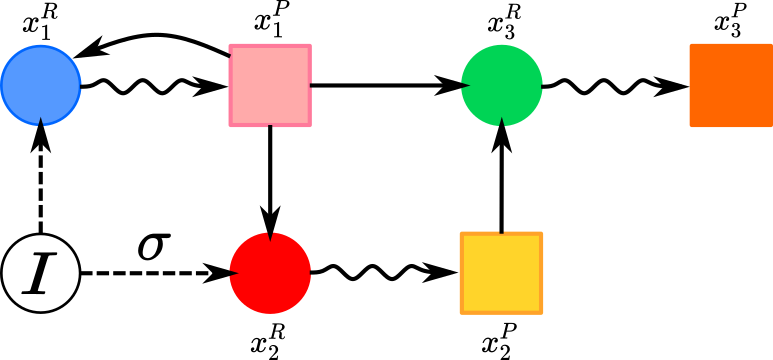
\includegraphics[scale=0.65]{figs/broken_n1_1.png}
    \caption{}
    \label{fig:broken_n1_two}
\end{figure}

The general admissible system of equations for this circuit differs from 
Eq.~\ref{eq:broken_n1_1} only in the dependence of the nonlinear function 
$f_{x_2^R}$, and it is given as
\begin{equation}
    \begin{aligned}
        \dot{x}_1^R &= f_{x_1^R}(x_1^R, x_1^P, \mathcal{I})\\
        \dot{x}_1^P &= f_{x_1^P}(x_1^P, x_1^R)\\
        \dot{x}_2^R &= f_{x_2^R}(x_2^R, x_1^P, \sigma \mathcal{I})\\
        \dot{x}_2^P &= f_{x_2^P}(x_2^P, x_2^R)\\
        \dot{x}_3^R &= f_{x_3^R}(x_3^R, x_1^P, x_2^P)\\
        \dot{x}_3^P &= f_{x_3^P}(x_3^P, x_3^R)
    \end{aligned},
\end{equation}

This time, the circuit has two input nodes and we cannot apply the same methodology
used before as we need to take into account the generalization of the theoretical 
framework presented in section~\ref{sec:intro} based on \cite{wang2021}. This 
generalization is described in \cite{multi_input_antoneli2020}. 


Therefore, 
we enumerate the proper classifications for the network of 
Fig.~\ref{fig:broken_n1_two} to find the general infinitesimal homeostasis 
conditions. First, we denote the input nodes $x_1^R \rightarrow I_1$
and $x_2^R \rightarrow I_2$, and the output node $x_3^P \rightarrow \mathcal{O}$.
Then, we have the following \textbf{$I_1\mathcal{O}$-simple paths}:
\begin{equation}
    \begin{aligned}
        I_1 &= x_1^R \rightarrow x_1^P \rightarrow x_3^R
        \rightarrow x_3^P = \mathcal{O}\\
        I_1 &= x_1^R \rightarrow x_1^P \rightarrow x_2^R
        \rightarrow x_2^P \rightarrow x_3^R \rightarrow x_3^P
        = \mathcal{O}
    \end{aligned},
\end{equation}
while we have one single \textbf{$I_2\mathcal{O}$-simple path}:
\begin{equation}
    I_2 = x_2^R \rightarrow x_2^P \rightarrow x_3^R
    \rightarrow x_3^P = \mathcal{O}.
\end{equation}

There are no appendage nodes, only simple nodes. Thus, we have 
$\{ x_1^R, x_1^P, x_2^R, x_2^P, x_3^R, x_3^P \}$ as $I_1$-simple 
nodes and $\{ x_2^R, x_2^P, x_3^R, x_3^P \}$ as $I_2$-simple 
nodes. Following the notation used in \cite{multi_input_antoneli2020}
we have that the \textit{absolutely super-simple nodes} are $x_3^R$ and 
$x_3^P$. Therefore, from these enumerations, we identify the 
\textit{absolutely super-simple structural} subnetwork 
$\mathcal{L'}(x_3^R, x_3^P)$ containing only $x_3^R$ and 
$x_3^P$. In principle, this subnetwork can allow only Haldane 
homeostasis, but following the special model used so far, the
factor $\det(H(\mathcal{L'}(x_3^R, x_3^P))) = f_{x_3^P,x_3^R} 
= \beta_3 \neq 0$. 
Moreover, we can also determine the \textit{input 
counterweight} subnetwork $\mathcal{W}_{\mathcal{G}}$ composed 
by nodes $\{ I_1 = x_1^R, I_2 = x_2^R, x_1^P, x_2^P, x_3^R \}$. 
The homeostasis type supported by this subnetwork is obtained 
from the determinant relation 
$det(H'(\mathcal{W}_{\mathcal{G}})) = 0$, where $H'$ is called
generalized homeostasis matrix. $H'$ can be obtained from the 
Jacobian $J_{\mathcal{W}_{\mathcal{G}}}$:
\begin{equation}
    J_{\mathcal{W}_{\mathcal{G}}} = 
    \begin{pmatrix}
        f_{x_1^R, x_1^R} & f_{x_1^R,x_1^P} & 0 & 0 & 0 \\
        f_{x_1^P, x_1^R} & f_{x_1^P, x_1^P} & 0 & 0 & 0 \\
        0 & f_{x_2^R, x_1^P} & f_{x_2^R, x_2^R} & 0 & 0 \\
        0 & 0 & f_{x_2^P, x_2^R} & f_{x_2^P, x_2^P} & 0 \\
        0 & f_{x_3^R, x_1^P} & 0 & f_{x_3^R, x_2^P} & f_{x_3^R, x_3^R} \\
    \end{pmatrix},
\end{equation} 
where for $H'(\mathcal{W}_{\mathcal{G}})$ the last column of 
$J_{\mathcal{W}_{\mathcal{G}}}$ is replaced by the column 
resulted from implicit differentiation, such that we have
\begin{equation}
    H'({\mathcal{W}_{\mathcal{G}}}) = 
    \begin{pmatrix}
        f_{x_1^R, x_1^R} & f_{x_1^R,x_1^P} & 0 & 0 & -f_{x_1^R, I} \\
        f_{x_1^P, x_1^R} & f_{x_1^P, x_1^P} & 0 & 0 & 0 \\
        0 & f_{x_2^R, x_1^P} & f_{x_2^R, x_2^R} & 0 & -f_{x_2^R, I} \\
        0 & 0 & f_{x_2^P, x_2^R} & f_{x_2^P, x_2^P} & 0 \\
        0 & f_{x_3^R, x_1^P} & 0 & f_{x_3^R, x_2^P} & 0 \\
    \end{pmatrix},
\end{equation} 
at the equilibrium point $(\vec{x}_0(I_0), I_0)$. According to 
\cite{multi_input_antoneli2020}, we can decompose 
$H'({\mathcal{W}_{\mathcal{G}}})$ into $m$ homeostasis matrices
\begin{equation}
    det(H'(\mathcal{W}_{\mathcal{G}})) = 
    \pm f_{x_1^R, I}det(H_1) \pm f_{x_2^R, I}det(H_2)
\end{equation}
where $m$ is the number of input nodes, and $H_i$ is the 
homeostasis matrix regarding the input node $I_i$. Here, we 
obtain the determinant of $H'$ directly, such that we have 
\begin{equation} \label{eq:det_n1_2input}
    \begin{split}
        det(H'(\mathcal{W}_{\mathcal{G}})) &=  
    -f_{x_2^R, I}f_{x_2^P,x_2^R}f_{x_3^R, x_2^P}
    (f_{x_1^R,x_1^R}f_{x_1^P, x_1^P} - 
    f_{x_1^R,x_1^P}f_{x_1^P,x_1^R}) \\ 
    &-f_{x_1^R,I}f_{x_1^P,x_1^R}
    (f_{x_2^R, x_1^P}f_{x_2^P,x_2^R}f_{x_3^R,x_2^P} + 
    f_{x_2^R,x_2^R}f_{x_2^P,x_2^P}f_{x_3^R,x_1^P}) = 0.
    \end{split}
\end{equation}

From Eq.~\ref{eq:det_n1_2input} we can recover the case 
worked in section~\ref{ssec:broken_n1} regarding the circuit 
receiving only one input by setting $\sigma = 0$. In this 
case, the infinitesimal homeostasis condition is given
by
\begin{equation} \label{eq:det_n1_2input1}
    \begin{split}
        det(H'(\mathcal{W}_{\mathcal{G}})) =  
    f_{x_1^R,I}f_{x_1^P,x_1^R}
    (f_{x_2^R, x_1^P}f_{x_2^P,x_2^R}f_{x_3^R,x_2^P} + 
    f_{x_2^R,x_2^R}f_{x_2^P,x_2^P}f_{x_3^R,x_1^P}) = 0
    \end{split},
\end{equation}
equivalent to the conditions obtained in section~\ref{ssec:broken_n1}
for which $f_{x_1^R,I} = 1$.

Considering the form of the Jacobian of the FFF circuit for the special
model given by Eq.~\ref{eq:jaco-special-1} and Eq.~\ref{eq:jaco-special-2},
we have that the condition of Eq.~\ref{eq:det_n1_2input} is 
\begin{equation}
    \begin{split}
        &-\sigma \beta_2 \gamma_3 T'(x_1^P + x_2^P) 
        \bigg[ \delta_1 \alpha_1 - \xi_1\beta_1\gamma_1 S'(x_1^P) \bigg] \\ 
        &-\beta_1 \bigg[ \xi_1\gamma_2\gamma_3\beta_2 S'(x_1^P)T'(x_1^P + x_2^P)
        + \delta_2\alpha_2\gamma_3 T'(x_1^P + x_2^P) \bigg] = 0
    \end{split},
\end{equation}
for the Jacobian $J_1$, while we obtain
\begin{equation}
    \begin{split}
        &-\sigma \beta_2 \gamma_3' S'(x_2^P) 
        \bigg[ \delta_1 \alpha_1 - \xi_1\beta_1\gamma_1 S'(x_1^P) \bigg] \\ 
        &-\beta_1 \bigg[ - \xi_1\gamma_2\gamma_3'\beta_2 S'(x_1^P)S'(x_2^P)
        + \delta_2\alpha_2\gamma_3 S'(x_1^P) \bigg] = 0
    \end{split},
\end{equation}
for the Jacobian $J_2$. Both conditions are calculated at $(\vec{x}_0(I_0), I_0)$.